\documentclass[10pt, pdf, hyperref={unicode}]{beamer}
\usepackage[T2A]{fontenc}
\usepackage[utf8]{inputenc}
\usepackage[english, russian]{babel}
\usepackage{amssymb, amsfonts, amsmath, amsthm, microtype, pdfpages}

\usetheme{Madrid}
\usecolortheme{beaver}

\title{<<Математическая модель импульсного погружателя, оптимального по коэффициенту асимметрии>>}
\date{10.06.2019}
\author{Уткин Артем Александрович}

\setbeamertemplate{frametitle}[default][center]
\setbeamertemplate{navigation symbols}{}
\setbeamertemplate{footline}[page number]


\begin{document}
    
    \begin{frame} % титульный лист 
        \titlepage
    \end{frame}


    \begin{frame}
        % \begin{figure}[h]
            % \begin{center}
                \begin{minipage}[h]{0.5\linewidth}
                    \frametitle{Описание вибрационного погружателя}
                    Вибрационный погружатель предназначен для погружения или извлечения свай в песчаных или глинистых грунтах.
                    \begin{block}{Определение 1}
                        Вибрационным погружением называют внедрение твердого тела в сопротивляющуюся среду под действием постоянной и знакопеременной сил.
                    \end{block}
                \end{minipage}
                \hfill 
                \begin{minipage}[h]{0.4\linewidth}
                    % \begin{block}{Схема вибрационного погружателя.}
                    %     \centering
                        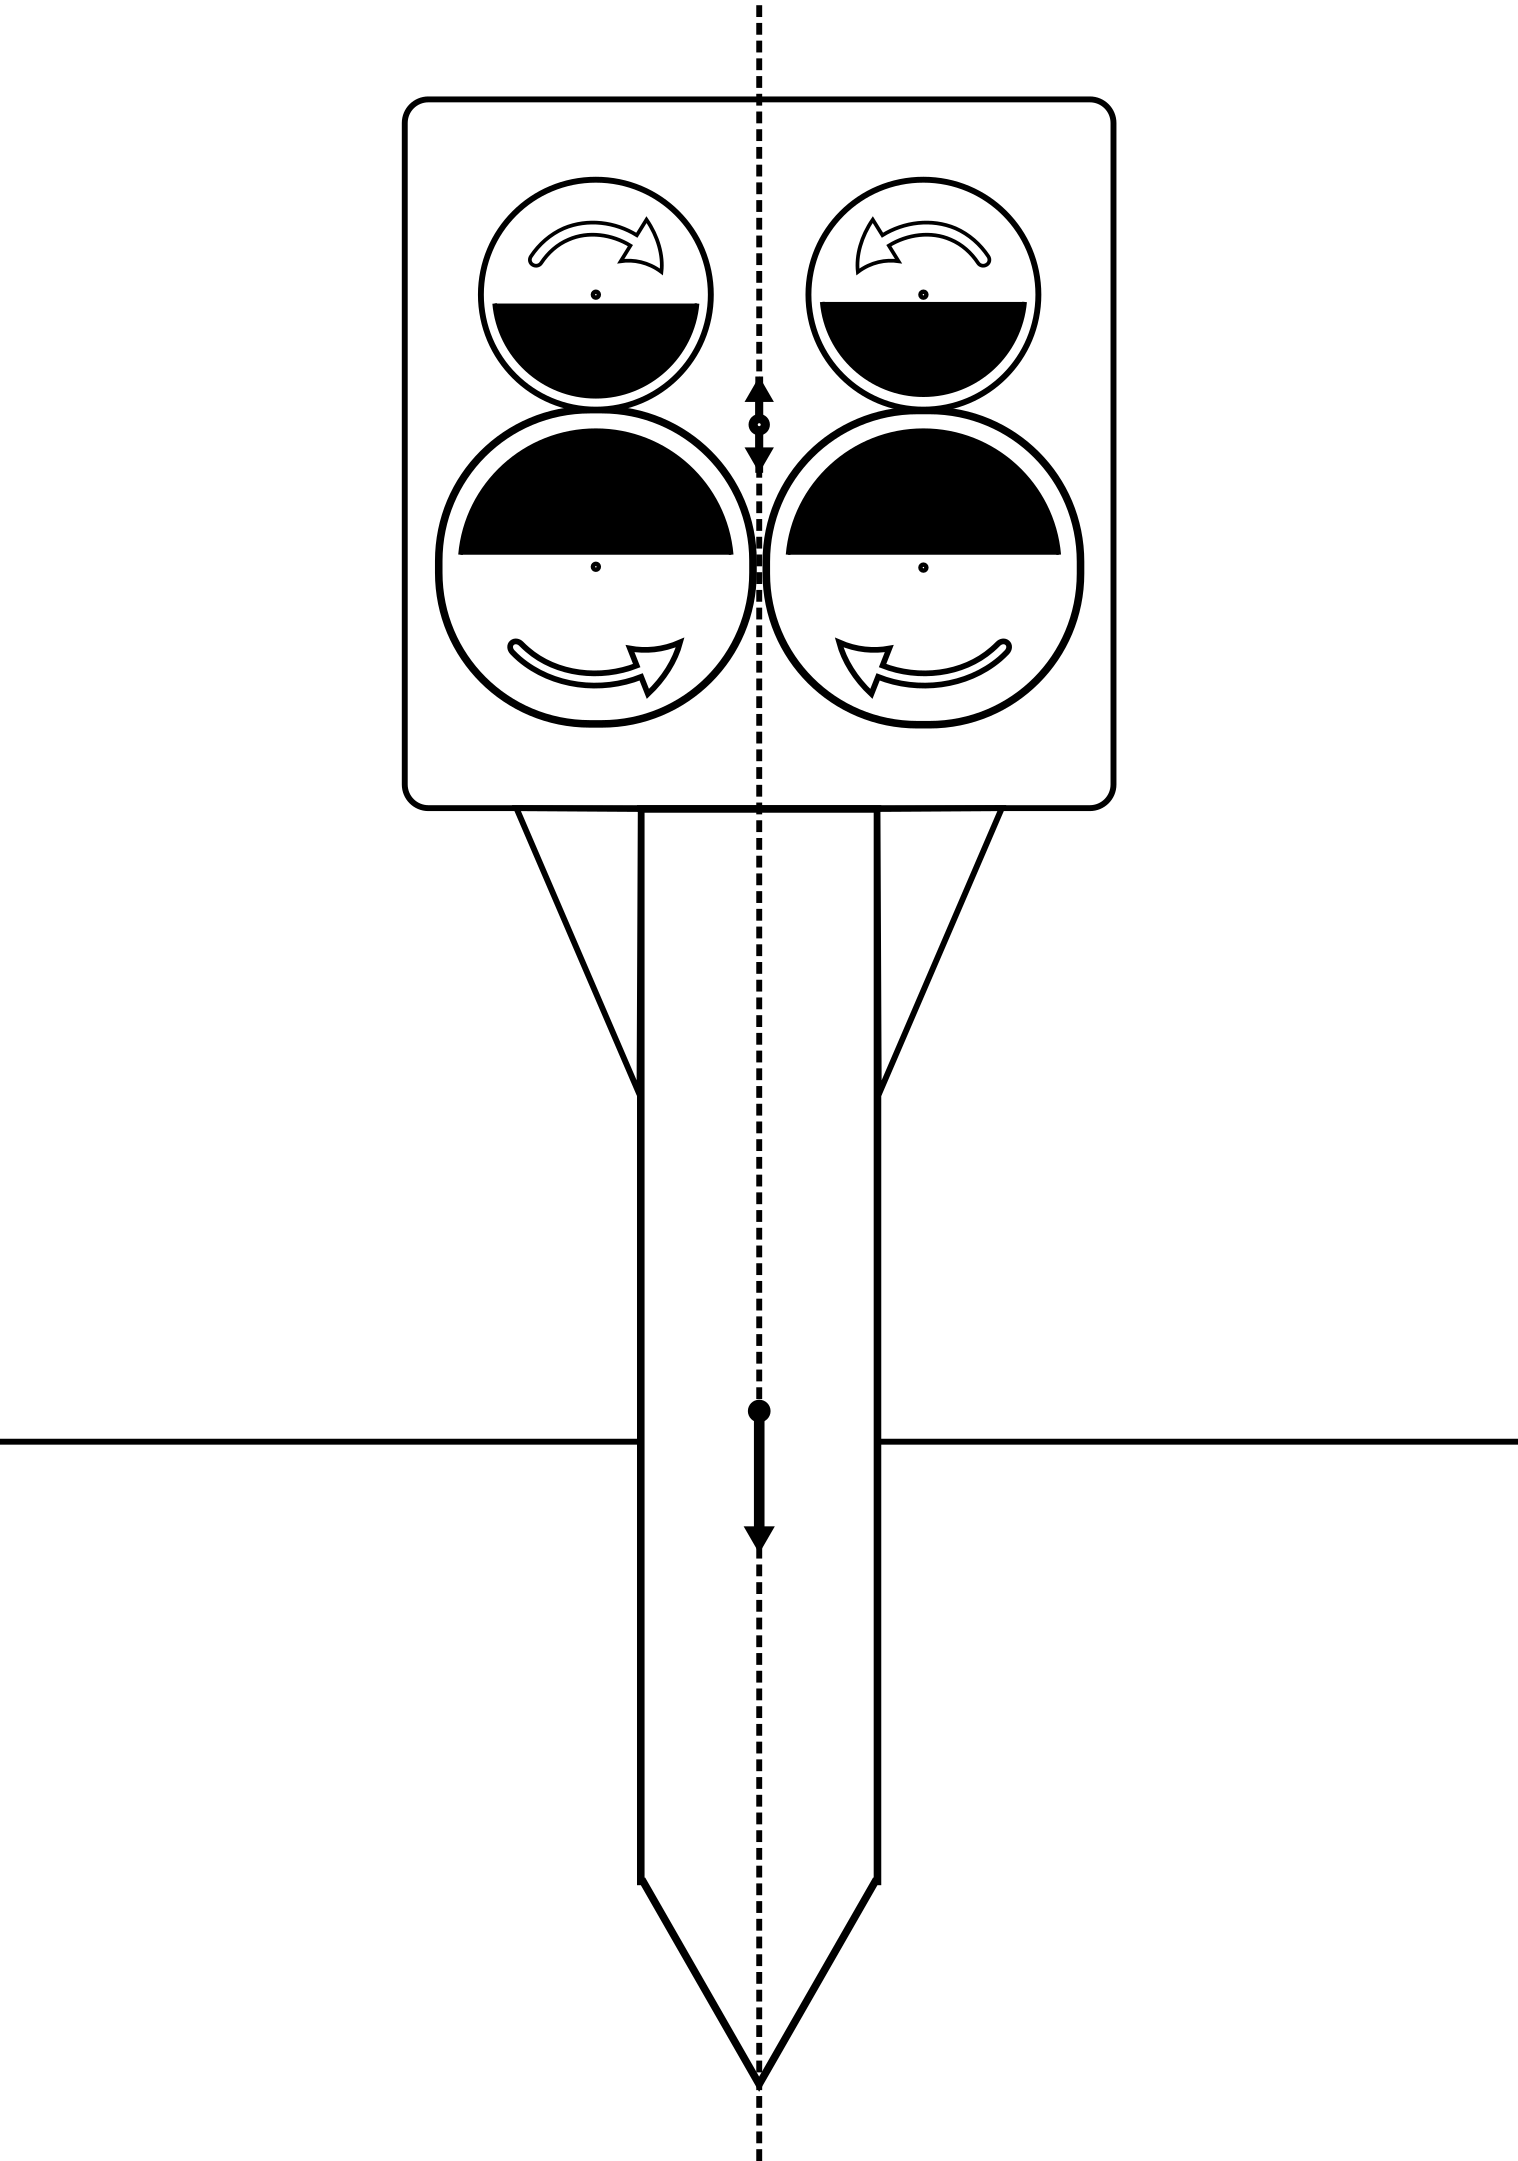
\includegraphics[width=1\linewidth]{../img/scheme_porg.png}
                        % \caption{Схема вибрационного погружателя.}
                        % \label{fig:scheme_porg}
                    % \end{block}
                \end{minipage}
            % \end{center}
        % \end{figure}
    \end{frame}


    \begin{frame}
        При вращении дебалансов на их ось крепления действует центробежная сила и вибрационный погружатель получает вибрирующее движение,
        которое сообщается свайному элементу через наголовник.
        
        \begin{block}{Определение 2}
            Дебалансом называют неуравновешенность вращающихся частей машин (роторов, коленчатых валов, шкивов и т. п.).
        \end{block}
        
        % \begin{block}{Определение 3}
        %     Сила, препятствующая материальной точке, движущейся по окружности, удалиться от центра этой окружности,
        %     называется центростремительной силой. Она направлена по радиусу от окружности к центру.
        %     По третьему закону Ньютона имеется равная ей и противоположно направленная сила противодействия
        %     (сила, с которой движущаяся точка стремится удалиться от центра). Эта сила называется центробежной.
        % \end{block}
    \end{frame}


    \begin{frame}
        \begin{minipage}[h]{0.48\linewidth}
            \begin{figure}[h]
                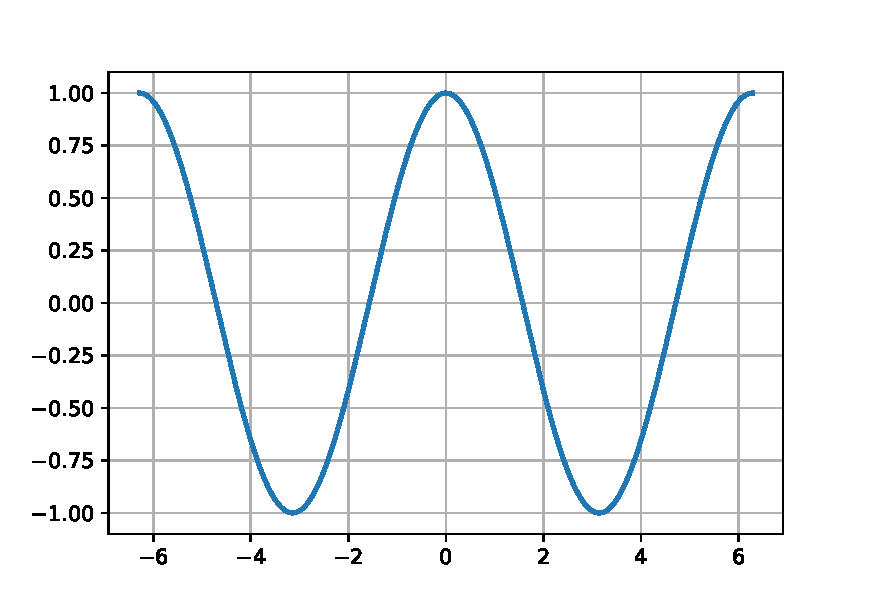
\includegraphics[width=1\linewidth]{../grap/impulse_1.pdf}
                \caption{График гармонических колебаний одной пары дебалансов.}
            \end{figure}
        \end{minipage}
        \hfill 
        \begin{minipage}[h]{0.48\linewidth}
            \begin{figure}[h]
                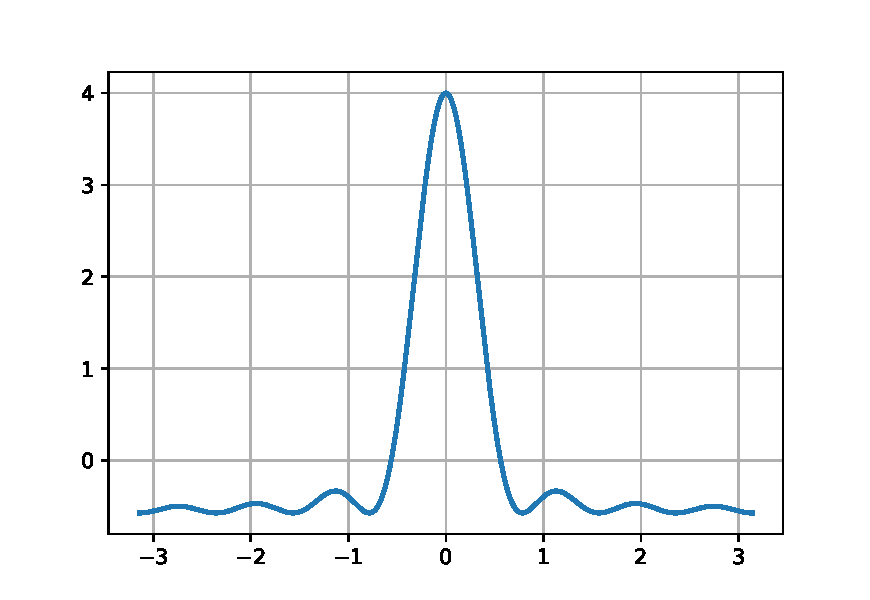
\includegraphics[width=1\linewidth]{../grap/impulse_7.pdf}
                \caption{График гармонических колебаний семи разных пар дебалансов.}
            \end{figure}
        \end{minipage}
    \end{frame}


    \begin{frame}
        \centerline{\large Спасибо за внимание!!!!!!!!11111111111111111111oneone}
    \end{frame}
\end{document}
